\documentclass[a4paper, 12pt]{article}

%%%%%%%%%%%%
% Packages %
%%%%%%%%%%%%

\usepackage[english]{babel}
\usepackage[noheader]{packages/sleek}
\usepackage{packages/sleek-title}
\usepackage{packages/sleek-theorems}
\usepackage{packages/sleek-listings}
\usepackage{booktabs}
\usepackage{verbatim}
\usepackage{listings}
\usepackage{xcolor}
\definecolor{mygreen}{rgb}{0,0.6,0}
\definecolor{mygray}{rgb}{0.5,0.5,0.5}
\definecolor{mymauve}{rgb}{0.58,0,0.82}
\lstset{ 
  backgroundcolor=\color{white},   % choose the background color; you must add \usepackage{color} or \usepackage{xcolor}; should come as last argument
  basicstyle=\ttfamily\scriptsize,        % the size of the fonts that are used for the code
  breakatwhitespace=false,         % sets if automatic breaks should only happen at whitespace
  breaklines=true,                 % sets automatic line breaking
  captionpos=b,                    % sets the caption-position to bottomhttps://www.overleaf.com/project/5e8f247c51e4ab0001a4aad8
  commentstyle=\color{mygreen},    % comment style
  deletekeywords={},            % if you want to delete keywords from the given language
  escapeinside={},          % if you want to add LaTeX within your code
  extendedchars=true,              % lets you use non-ASCII characters; for 8-bits encodings only, does not work with UTF-8
  firstnumber=1000,                % start line enumeration with line 1000
  frame=none,	                   % adds a frame around the code
  keepspaces=true,                 % keeps spaces in text, useful for keeping indentation of code (possibly needs columns=flexible)
  columns=fullflexible,
  keywordstyle=\color{black},       % keyword style
  language=python,                 % the language of the code
  morekeywords={*,...},            % if you want to add more keywords to the set
  numbers=none,                    % where to put the line-numbers; possible values are (none, left, right)
  numbersep=5pt,                   % how far the line-numbers are from the code
  numberstyle=\tiny\color{mygray}, % the style that is used for the line-numbers
  rulecolor=\color{black},         % if not set, the frame-color may be changed on line-breaks within not-black text (e.g. comments (green here))
  showspaces=false,                % show spaces everywhere adding particular underscores; it overrides 'showstringspaces'
  showstringspaces=false,          % underline spaces within strings only
  showtabs=false,                  % show tabs within strings adding particular underscores
  stepnumber=2,                    % the step between two line-numbers. If it's 1, each line will be numbered
  stringstyle=\color{mymauve},     % string literal style
  tabsize=5,	                   % sets default tabsize to 2 spaces
  title=\lstname                   % show the filename of files included with \lstinputlisting; also try caption instead of title
}
\hypersetup{
    colorlinks = true,
    linkcolor = black,
    anchorcolor = black,
    citecolor = black,
    filecolor = black,
    urlcolor = black
    }
\usepackage{longtable}

%%%%%%%%%%%%%%
% Title-page %
%%%%%%%%%%%%%%

\logo{./resources/image/logo.png}
\institute{Politecnico di Torino}
\faculty{Computer engineering}
\department{Department of Computer Engineering, \linebreak Cinema and Mechatronics}
\title{SSD Object Detection Model for Blender Gestural Input Interface}
\subtitle{Course of Machine Learning for Vision and Multimedia}
\author{\textit{s286312}\quad Marzio\quad \textsc{Vallero}\linebreak}

\supervisor{Professors\linebreak
            Fabrizio \textsc{Lamberti}\linebreak
            Lia \textsc{Morra}\linebreak}

\date{a.y. 2021/2022}

%%%%%%%%%%%%%%%%
% Bibliography %
%%%%%%%%%%%%%%%%

%%%%%%%%%%
% Others %
%%%%%%%%%%
\lstdefinestyle{latex}{
    language=TeX,
    style=default,
    %%%%%
    commentstyle=\ForestGreen,
    keywordstyle=\TrueBlue,
    stringstyle=\VeronicaPurple,
    emphstyle=\TrueBlue,
    %%%%%
    emph={LaTeX, usepackage, textit, textbf, textsc}
}

\FrameTBStyle{latex}

\def\tbs{\textbackslash}

\usepackage[nottoc]{tocbibind}

%%%%%%%%%%%%
% Document %
%%%%%%%%%%%%

\begin{document}
\maketitle
\twocolumn
\sloppy

\section{Abstract}
\begin{flushleft}
This paper aims at describing the steps required for the training of a custom purpose Object Detector neural network to be used as a mean of interaction for the 3D modeling software Blender. The first part will describe the generation of a custom dataset for training over hand gestures containing images of a single person, explaining techniques used to reduce as much as possible any bias due to this.\linebreak
This dataset will be then used to transfer learn a Single Shot Multibox Detector with Feature Pyramid architecture through Tensorflow's Object Detection API.
The results will be evaluated through training statistics and direct experimentation with the trained model, discussing about the approaches used and possible improvements.
Results and code relative to this paper are available at the project's \href{https://github.com/MarzioVallero/ML-Based-Blender-Gestural-Input-Interface}{GitHub page}.
\end{flushleft}

\section{Introduction}
\begin{flushleft}
Most of modern era 3D software human-computer interfaces rely onto the usage of a mouse and a keyboard. This can prove to be a difficult task to learn, as this mean of manipulation can seems daunting and complex for newcomers.\linebreak
It has been proven already in \hyperref[Ref4]{[7]} that Engineering Graphics are amongst the most difficult tasks to fully grasp for students and that 3D simulated environments improve their learning capabilities.\linebreak
This paper aims at detailing the steps required to create an object detection neural network able to recognize static hand gestures. Such network is a Single Shot Multibox Detector \hyperref[Ref1]{[4]}, designed by Google Brain researchers as seen in \hyperref[RefSSD]{[1]}, and trained on Microsoft's COCO 17 dataset (\hyperref[Ref2]{[5]}). Its checkpoints are publicly available through \hyperref[Ref10]{[10]}.\linebreak
The project will first introduce the steps for the generation of a custom dataset for training, applying data augmentation and negative samples. This is done to reduce the bias due to the fact that it contains only images of the same person. This dataset will then be used to train through transfer learning (\hyperref[Ref3]{[6]}) a checkpoint of the SSD and discuss about training statistics and experimental results.\linebreak
This input interface could see applications as an instrument for learning (molecules, human body models or mechanical models) and as a mean of interaction in museums or during large-scale presentations.
\end{flushleft}

\section{Dataset}
\begin{flushleft}
The first step amounts to the generation of the custom dataset, justified by the fact that no current dataset exists containing all of the gestures we wanted to use.
In order to do so, we followed the steps which are also described in the Python Notebooks \href{https://github.com/MarzioVallero/ML-Based-Blender-Gestural-Input-Interface/blob/master/DatasetGeneration.ipynb}{DatasetGeneration.ipynb}.\linebreak
This step is responsible for the definition of the set of gestures and for automated sample capture. After defining the number of images we want to collect for each object class, we proceed to actually capture the frames, which are automatically saved in separate directories according to their label of reference. It is recommended to produce for each label the same amount of samples and to insert a single gesture per frame.\linebreak
The amount of data at the network's disposal for training greatly impacts its ability to learn: for this very reason, we exploited data augmentation to increase the number of available samples for the network whilst trying to reduce the implicit bias due to having a single person produce the whole dataset. The data augmentation transformations used are horizontal/vertical stretching and zooming. Other data augmentation techniques could have caused shape overlaps between gestures and have thus been avoided. Negative samples have been introduced to reduce the amount of false positives registered by the network.\linebreak
Totally, we defined 12 classes, plus an extra unlabeled one for negative samples. For each class, we produced 100 samples.\linebreak
The main variance between sets of images for the same label were different spatial positions of the hand with respect to the frame and rotations of the wrist.\linebreak
It's important to note that a wider dataset for each gesure will increase variance, increasing accuracy and the generalization capabilities of the final trained model.

The labeling process has been done with \textit{\hyperref[Ref11]{LabelImg}}, a python based graphic tool that lets us manually select a region of interest within each frame and label it according to a specific class.
This process produces, for each frame, an output \textit{.xml} file that embeds the coordinates of the region of interest and label of a specific frame. At the end of the process, we will have an \textit{.xml} for each frame of the dataset. The negative samples will have and empty \textit{.xml} file, generated by pressing \textit{Verify Image} on LabelImg's GUI.\linebreak

\begin{figure}[!h]
    \centering
    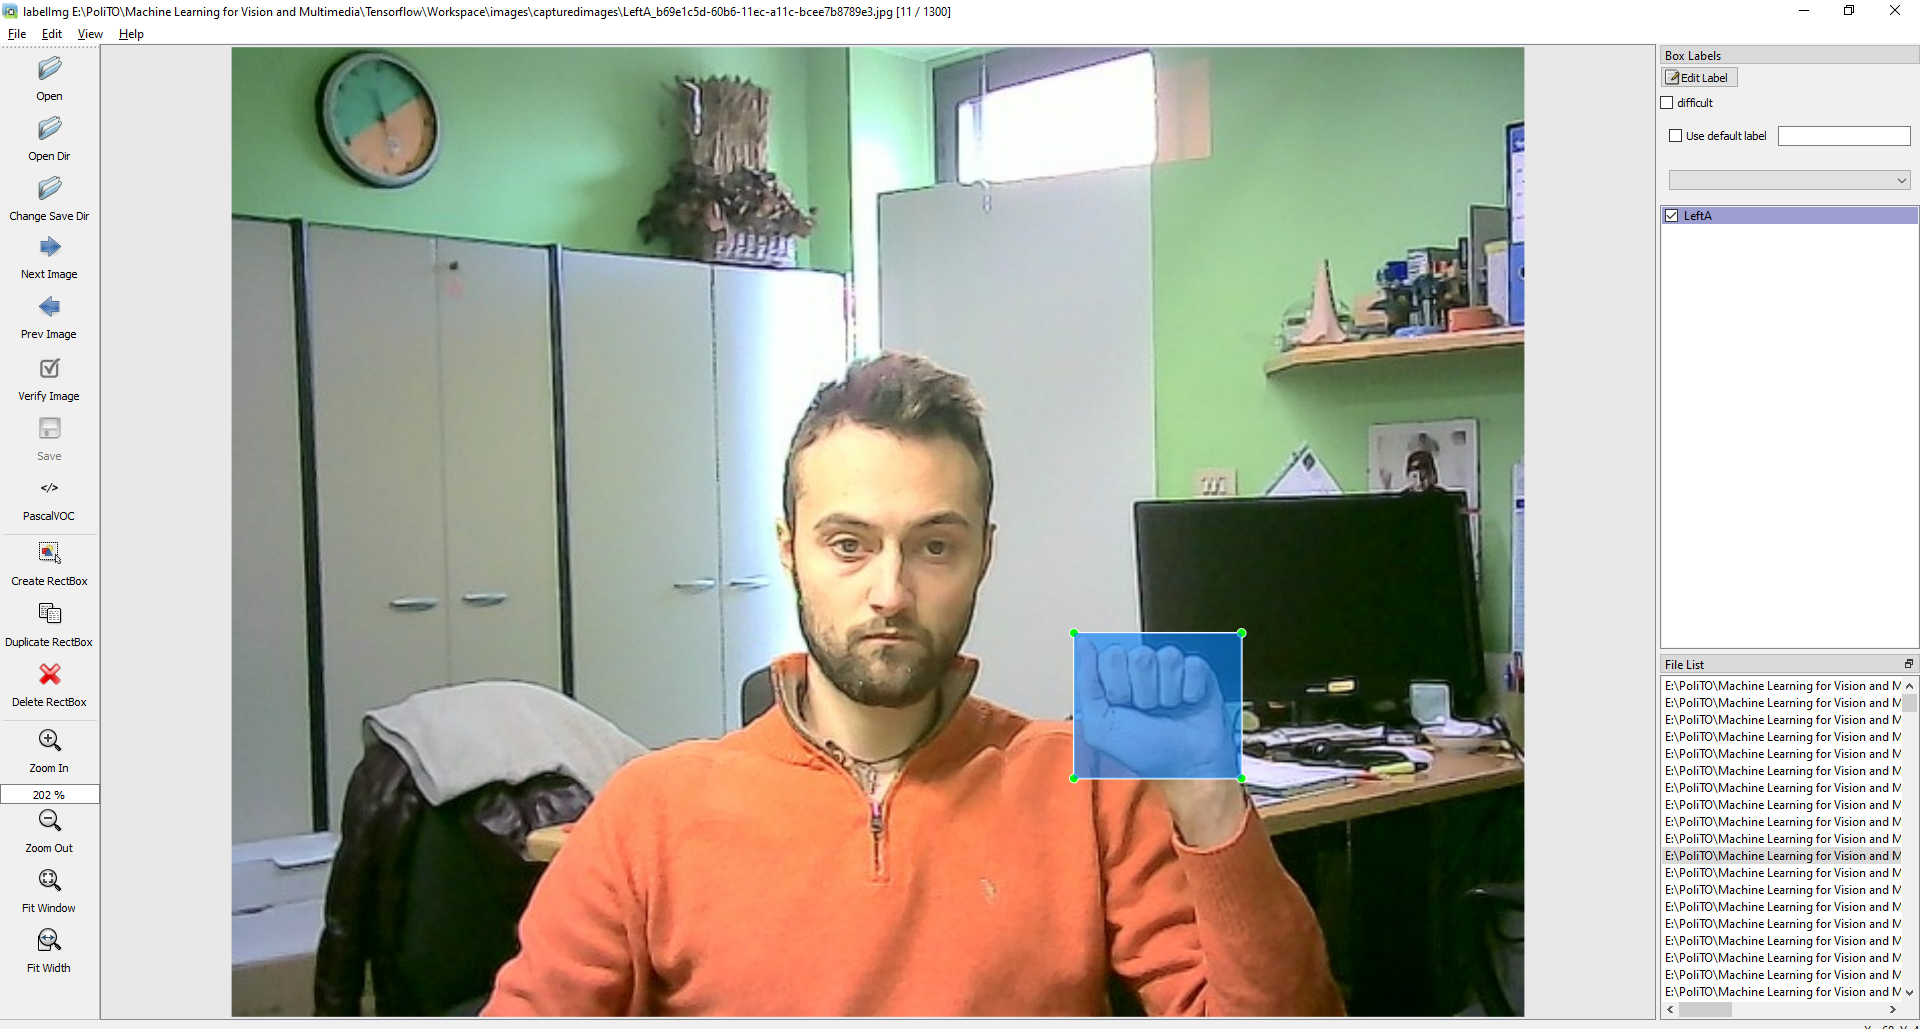
\includegraphics[width=0.5\textwidth]{resources/image/labelImgScreenshot.PNG} \caption{The LabelImg interface after drawing a bounding box around a gesture.}
\end{figure}

The final dataset thus contains $1300$ images representing the same person, on the same background, doing a total of 12 different gestures. It has been split into two partitions, with 25\% for testing and 75\% for training.
\end{flushleft}

\section{Methods}
\begin{flushleft}
The first approach we though of for creating an input interface for Blender was to build and train a RNN able to recognize actions from a video input. This however proved to be extremely inadequate in terms of usability, since repeating an action multiple times was the only way to produce incremental transformations through the interface. Moreover, the task of generating and labeling a custom dataset for such approach would have had a big impact on the time available for the project's development. For this reason this approach was ultimately discarded.\linebreak
The second approach, which was later adopted, was to train an Object Detection network able to map continuous static input gestures to transformations in the 3D scene of Blender. The choice of using the SSD MobileNet V2 FPNlite network arised from its inherent state of the art characteristics: a very fast mean input processing time of 22 ms, which suits perfectly the need to process video at 30 FPS from a webcam, which generates an image every 33.3 ms and its very high mAP score of 22.2 onto the COCO 17 dataset on which it was initially trained.\linebreak
This approach moreover let us apply transfer learning to retrain a pre-existing model, improving considerably the required training times.
The chosen model was originally developed by Google Brain researchers in \hyperref[Ref1]{[4]} and aimed at improving over current hand-crafted CNNs, learning a better architecture of feature pyramid network for object detection, called NAS-FPN. The main changes applied to such network were the removal of the \textit{random\_horizontal\_flip} data augmentation layer and the reduction of total training steps, justified by the fact that the dataset we used is much smaller with respect to COCO 17 and thus boasts less features to be learnt.\linebreak

The model's architecture is explained in detail in the developer's paper \hyperref[RefArchSSD]{[2]}.
The basic building block introduced in their paper is a bottleneck depth-separable convolution layer with residuals, whose structure is shown in \hyperref[figure2]{Figure 2}.

\begin{figure}[!h]
    \centering
    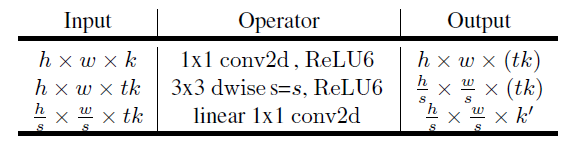
\includegraphics[width=0.5\textwidth]{ML Project/resources/image/MoblieNetV2Table1.png} \caption{Bottleneck residual block transforming from k to k' channels, with stride s, and expansion factor t.}
\end{figure}
\label{figure2}

The general architecture of the model contains an initial fully convolutional layer with 32 filters, followed by 19 residual bottleneck layers described, as shown in Figure 3. The kernel size is 3 × 3, and dropout and batch normalization layers are used during training.

\begin{figure}[!h]
    \centering
    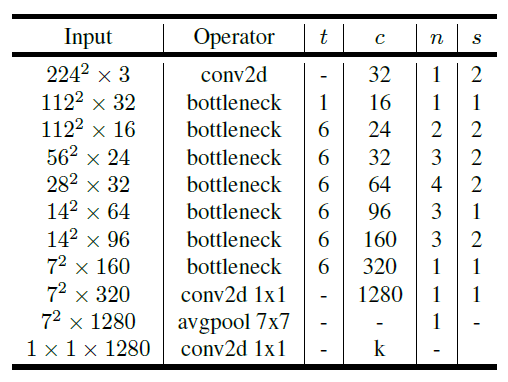
\includegraphics[width=0.5\textwidth]{ML Project/resources/image/MoblieNetV2Table2.png} \caption{The full model's architecture. Each line represents n repetitions of the same layer. All layers feature the same number of channels c. The first sequence layer has stride s, whilst the others have stride 1.}
\end{figure}
\label{figure3}

This architecture is then wrapped between six \textit{bottom\_up\_conv\_2d} layers and a \textit{FeatureMap} layer, as shown in figure 4.
As we can see, this version of the model features $2,223,872$ trainable parameters and $34,112$ non-trainable ones.\linebreak

\begin{figure}[!h]
    \centering
    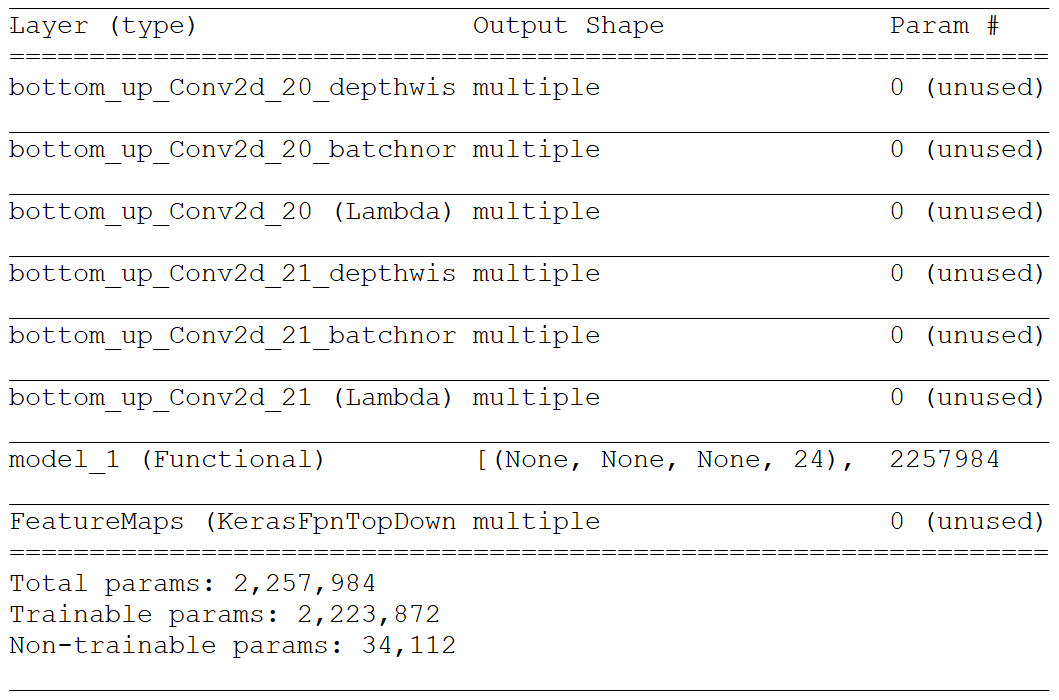
\includegraphics[width=0.5\textwidth]{ML Project/resources/image/architecture.PNG} \caption{The wrapped model's architecture, complete with parameters.}
\end{figure}
\label{figure4}

The loss used for training is split into four elements: classification, localization, regularization and total loss.
Classification loss refers to the model's ability to correctly predict an object's class and uses as loss function a weighted sigmoid focal, with gamma equal to 2 and alpha equal to 0.25.
Localization loss refers to the ability to find the position of the bounding box of an object inside the input image and uses as loss function a weighted smooth L1.
Regularization loss is an additional loss generated by the L2 regularization function, which gets added to the network's loss and used to optimize over the sum of the other two. This method is used to help the optimization algorithm to generalize better over the dataset.
The total loss represents the sum of these three previous losses and gives a top-down view of the model's training performance.\linebreak

The model's live performance has then been evaluated through the \href{https://github.com/MarzioVallero/ML-Based-Blender-Gestural-Input-Interface/blob/master/ModelTest.ipynb}{ModelTest.ipynb} notebook, checking the predicted labels superimposed over the input frames.\linebreak
To boost the model's prediction accuracy, we tried to apply HSV skin tone thresholding to remove most false positives and stabilizing the model's performance in the wild. The results were extremely encouraging and thus we kept this preprocessing step in the final evaluation script.

\end{flushleft}

\section{Experiments}
\begin{flushleft}
All the models have been trained onto a machine equipped with an \textit{Intel i5-11600K} CPU and accelerated through an \textit{NVidia GeForce RTX 2060 6GB} GPU.
The first training has been done over $20000$ steps, with a batch size of $8$, totaling $82$ epochs, and required over two hours to complete: this produced a model with a final Total Loss of $0.12568491$, still too high to provide stable predictions. Testing this checkpoint in fact proved to be unfeasible, as it was not able to recognize almost anything at all during the evaluation phase.
The training has then been resumed for another $20000$ steps, requiring another two hours and a half. The final Total Loss came out to be $0.09876089$, which is a great improvement over previous iterations. However, testing the model live immediately gave rise to bounding box detection issues and general inaccuracy of the predictions, without much generalization capabilities. Moreover, since the network during training internally performed horizontal flips for data augmentation, the left and right hand gestures got often swapped or overlapped. To boost the accuracy of the network, we threshold its input using an HSV profile, customizable to better suit each user.
To solve the hand swapping issue, we retrained the model once again and removed the horizontal flipping data augmentation layer, with a batch size of $16$, totaling $328$ epochs. This last training required only four hours and a half to complete, suggesting that we weren't fully exploiting the GPU before.
The training statistics for this last model are shown in \hyperref[figure5]{Figure 5}.
\begin{figure}[!h]
    \centering
    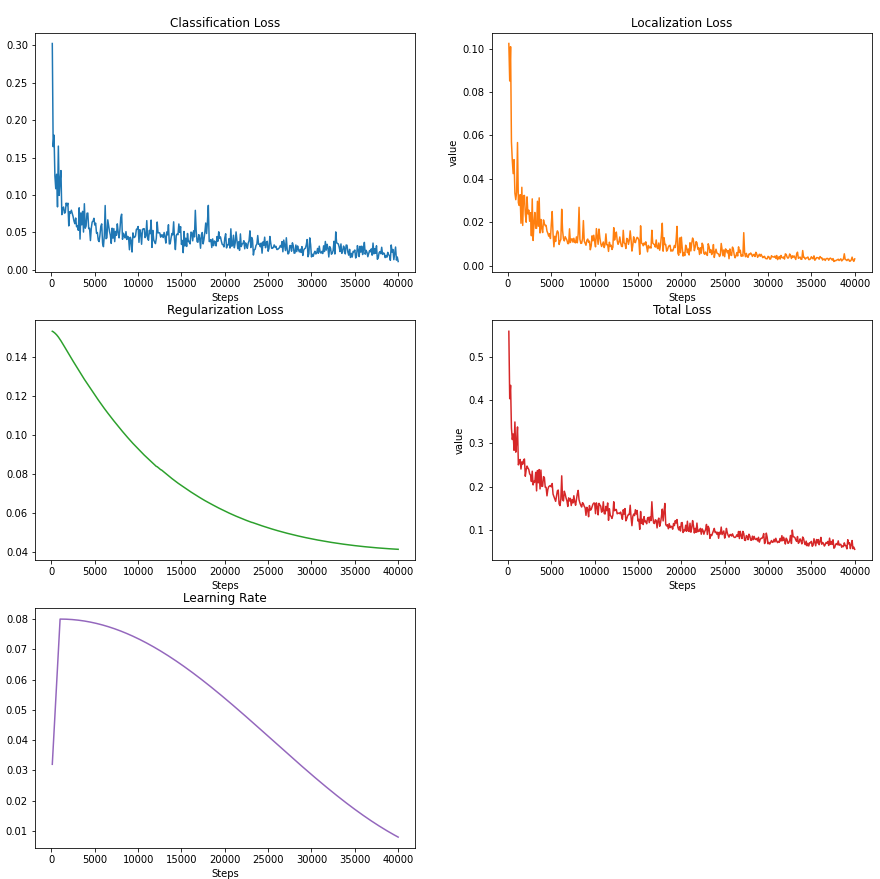
\includegraphics[width=0.5\textwidth]{ML Project/resources/image/statistics.PNG} \caption{All losses and learning rate statistics for the 40000 steps model trained without the horizontal flip data augmentation layer.}
\end{figure}
\label{figure5}
The role of the HSV thresholding preprocessing step plays an impactful role on the model's ability to process the input frames. Despite the fact that the dataset contains images with hands in different spatial positions over a complex background, the model sometimes produces random false positives, detecting a gesture where there is none. This may be due to the fact that the whole dataset contains the same static background, or that some of the features learnt by the network are edge bound and some objects happen to fit partially those feature requirements. However, after thresholding, most of the background contains no data, as shown in \hyperref[figure6]{Figure 6}, and thus gives to the model less room for error in evaluating gestures, often resulting in confidence measures of around 95\%-99\%.

\begin{figure}[!h]
    \centering
    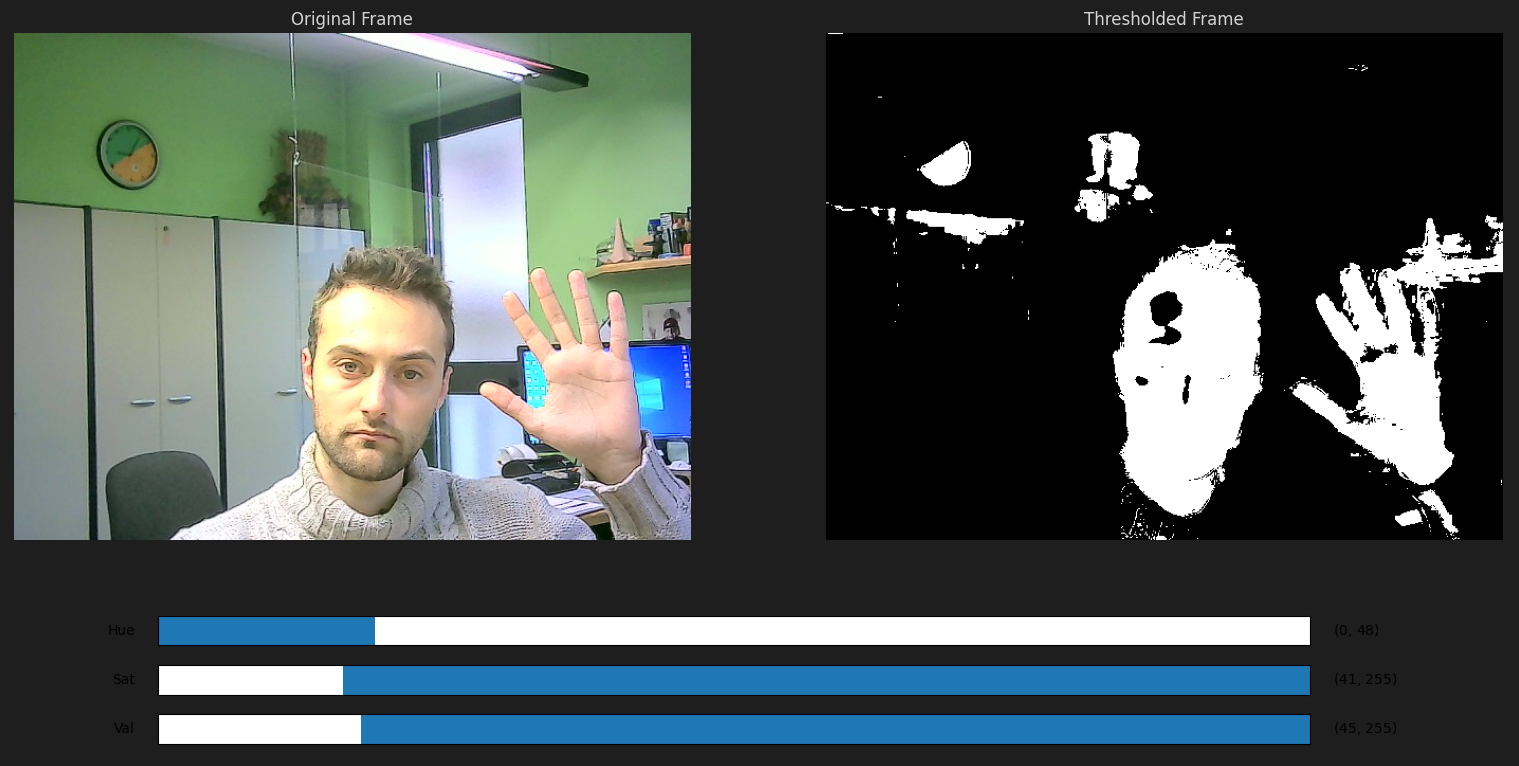
\includegraphics[width=0.5\textwidth]{ML Project/resources/image/thresholding.PNG} \caption{The effect of thresholding, as seen thorugh the \textit{\href{https://github.com/MarzioVallero/ML-Based-Blender-Gestural-Input-Interface/blob/master/CreateHSVProfile.py}{CreateHSVProfile.py}} script.}
\end{figure}
\label{figure6}

\end{flushleft}

\section{Conclusions}
\begin{flushleft}
The process of producing and understanding the model presented in this paper has been multi-faceted and long, however it also proved to be a very formative experience.\linebreak
The generation of the dataset has been a quite daunting task, requiring multiple days of work just for capturing and labeling. Moreover, the expansion of the dataset to include also negative samples to feed to the network resulted into a better generalization of the gesture features, reducing by a significant margin the false positives due to predicting gestures where there are none. In fact, one of the most common pitfalls in these kinds of applications is the false prediction of a hand gesture on the user's face, which in our case has been mitigated quite well.\linebreak
Setting up the \textit{pipeline.config} file proved to be a challenging task too, due to the required installation of the Tensorflow Object Detection API, which brought in many versioning issues deriving from Tensorflow 1 and 2 incompatible calls among the \textit{Tensorflow/models} submodule's scripts. In the end, parts of those scripts had to be modified by us in order to account for updates in Tensorflow's API.\linebreak
The analysis of the \textit{pipeline.config} file also gave us insight about the inner workings of the model, letting us tinker around hardware specific definitions to improve training performance (like the batch size, which we found out to boast better performance at value 16) and removing components which were working against our needs.\linebreak
The model's generalization capabilities over the single-person dataset proved to be extremely promising when evaluated onto different people. The model expects a certain shape and orientation, thus incorrect gestures due to different individual's interpretation still get unrecognized, though gestures which try to resemble more the original dataset end up being recognized with no issue and a high confidence of around 90\%. This requires a bit of effort from the user's side to work, however we believe it to be a quite encouraging result given the amount of data at our disposal. This aspect could be improved by generating a bigger dataset with higher user variance, especially in terms of hand morphology and skin tone, and consequently training for a higher number of steps.\linebreak
The thresholding external preprocessing step, originally implemented following \hyperref[Ref0]{[3]} as a \textit{YCbCr} thresholding, proved to boast low masking capabilities with respect to skin tone. It has later been changed to the current \textit{HSV} thresholding script, as allows for more precise masking for \textit{in-the-wild} environments.\linebreak
In conclusion, we believe the results of this paper to be significant, in that they provide insight over the techniques and approaches to be used to produce gestural input interfaces through the exploitation of Object Detector Neural Networks.\linebreak

\end{flushleft}

\onecolumn

\section{References}
\label{References}
\begin{flushleft}
\begin{enumerate}
    \item \label{RefSSD} \href{https://arxiv.org/pdf/1904.07392}{Golnaz G., Tsung-Yi L., Ruoming P., Quoc V.L.: NAS-FPN: Learning Scalable Feature Pyramid Architecture for Object Detection. 2019.}
    \item \label{RefArchSSD} \href{https://arxiv.org/pdf/1801.04381.pdf}{Sandler M., Howard A., Zhu M., Zhmoginov A., Chen L.C.: MobileNetV2: Inverted Residuals and Linear Bottlenecks. 2019.}
    \item  \label{Ref0} \href{https://ieeexplore.ieee.org/document/7916786}{Referring only onto the Skin Tone Segmentation section: Nikam A.S., Ambekar A.G.: Sign language recognition using image based hand gesture recognition techniques. 2016.}
    \item \label{Ref1} \href{https://arxiv.org/abs/1512.02325}{Liu W., Anguelov D., Erhan D., Szegedy C., Reed S., Fu C., Berg A. C.: Single Shot MultiBox Detector}. 2016.
    \item \label{Ref2} \href{https://arxiv.org/abs/1405.0312}{Lin T., Maire M., Belongie S., Bourdev L., Girshick R., Hays J., Perona P., Ramanan D., C. Zitnick L., Dollár P.: Microsoft COCO: Common Objects in Context}. 2015.
    \item \label{Ref3} \href{https://arxiv.org/abs/1911.02685}{Zhuang F., Qi Z., Duan K., Xi D., Zhu Y., Zhu H., Xiong H., He Q.: A Comprehensive Survey on Transfer Learning}. 2020.
    \item \label{Ref4} \href{https://ieeexplore.ieee.org/document/7814839}{Mavinkurve U., Verma D.: EG-Easy: Design and Testing of Blender-Based Tool to Teach Projections in Engineering Drawing. 2016 IEEE Eighth International Conference on Technology for Education (T4E), 2016, pp. 250-251, doi: 10.1109/T4E.2016.064.}
    \item \label{Ref8} \href{https://tensorflow-object-detection-api-tutorial.readthedocs.io/en/latest/}{Tensorflow Object Detection API installation}
    \item \label{Ref9} \href{https://github.com/tensorflow/models/tree/master/research/object_detection}{Tensorflow Object Detection API GitHub}
    \item \label{Ref10} \href{https://github.com/tensorflow/models/blob/master/research/object_detection/g3doc/tf2_detection_zoo.md}{TensorFlow 2 Detection Model Zoo}
    \item \label{Ref11} \href{https://github.com/tzutalin/labelImg}{LabelImg GitHub}
\end{enumerate}
\end{flushleft}

\end{document}